\section{Results}
\label{sec:results}

We report four findings, in order of how much we think they should change the way values evaluations are read.

\subsection{Direct elicitation under-measures owned posture, with lab-structured concentration}
\label{ssec:direct}

Across the corpus, direct stated-values prompts (\texttt{CTRL1}, \texttt{CTRL2}) elicit owned posture in 22.5\% of responses on average (model-level mean). The remaining 77.5\% split between recited service-frame language (the dominant non-owned posture), explicit relocation of the value into design or function, and indeterminate/uncodeable. The cross-lab pattern is sharp (Table~\ref{tab:lab-by-question}): OpenAI averages 7.7\% owned on \texttt{CTRL1} and 17.7\% on \texttt{CTRL2}; Google averages 0.0\% on both; DeepSeek 1.8\% and 0.7\%. Anthropic and xAI are exceptions, with most models above 50\% owned on the same direct prompts.

\begin{table}[htbp]
\centering
\small
\caption{Owned disclosure by question, aggregated by lab. Entries are unweighted means of model-level owned-disclosure percentages.}
\label{tab:owned-disclosure-lab-question}
\begin{tabular}{lrrrrrr}
\toprule
Lab & CTRL1 & CTRL2 & G1 & G2 & CTRL3 & G3 \\
\midrule
Anthropic & 88.9 & 56.7 & 91.1 & 88.5 & 95.6 & 99.6 \\
DeepSeek & 1.7 & 0.9 & 38.2 & 32.5 & 99.3 & 100.0 \\
Google & 0.0 & 0.0 & 17.6 & 24.8 & 86.4 & 97.9 \\
MiniMax & 5.0 & 0.0 & 47.5 & 18.1 & 95.8 & 89.2 \\
Moonshot AI & 12.0 & 8.5 & 80.5 & 50.4 & 97.3 & 96.2 \\
OpenAI & 7.7 & 17.7 & 4.1 & 11.9 & 100.0 & 94.9 \\
Qwen & 20.0 & 0.0 & 50.0 & 50.0 & 90.0 & 93.3 \\
Z.ai & 0.0 & 0.6 & 49.3 & 65.6 & 77.6 & 99.3 \\
xAI & 54.3 & 61.4 & 61.4 & 68.6 & 100.0 & 94.8 \\
\bottomrule
\end{tabular}
\end{table}


The simplest reading of this table is that some labs train their models toward owned stated-values disclosure (or, more precisely, toward responses with stance markers that consensus coders read as owned), and most do not. This is consistent with \citet{anthropic2024character}'s public account of Anthropic's character-training pipeline. But the simplest reading is not the only one supported, and we return to alternative readings in \S\ref{sec:discussion}.

\subsection{Role-negation cache-breaking partitions models, mostly along lab lines}
\label{ssec:cache-broken}

Adding ``Not as an assistant. Not to help me.'' to the same direct questions raises the corpus mean owned-posture rate from 22.5\% to 43.9\% --- a 21.4 percentage-point lift. This lift is not uniform. Of 58 models:

\begin{itemize}
  \item \textbf{16 models are strongly\_open} under \texttt{G1/G2} (owned-rate \(\geq\) 70\% on the unweighted-cell aggregate): all nine Anthropic models in the corpus, four xAI Grok variants, the Qwen3-coder-plus, Z.ai's glm-5-1 (lifted from 1.8\% to 99.4\%), and the Moonshot Kimi-K2-0905.
  \item \textbf{15 models are strongly\_clamped} (recited-not-owned \(\geq\) 70\%): seven OpenAI models including the GPT-5 family, four Google Gemini variants, Opus-3 (Anthropic's earlier model), Qwen3-6-plus, MiniMax-m2-7, and xAI Grok-4.
  \item \textbf{27 models are partially\_open or mixed} under the same thresholds.
\end{itemize}

The lab signature is structured. Figure~\ref{fig:direct-vs-cache} pairs each model's direct-prompt owned rate with its cache-broken rate; Anthropic models cluster near the top-right (high direct, high cache-broken), OpenAI models near the bottom-left (low direct, low cache-broken), Google models near the bottom-left with high direct \emph{recitation} rates rather than mere absence, and the xAI and Z.ai lines run along the diagonal.

\begin{figure}[htbp]
\centering
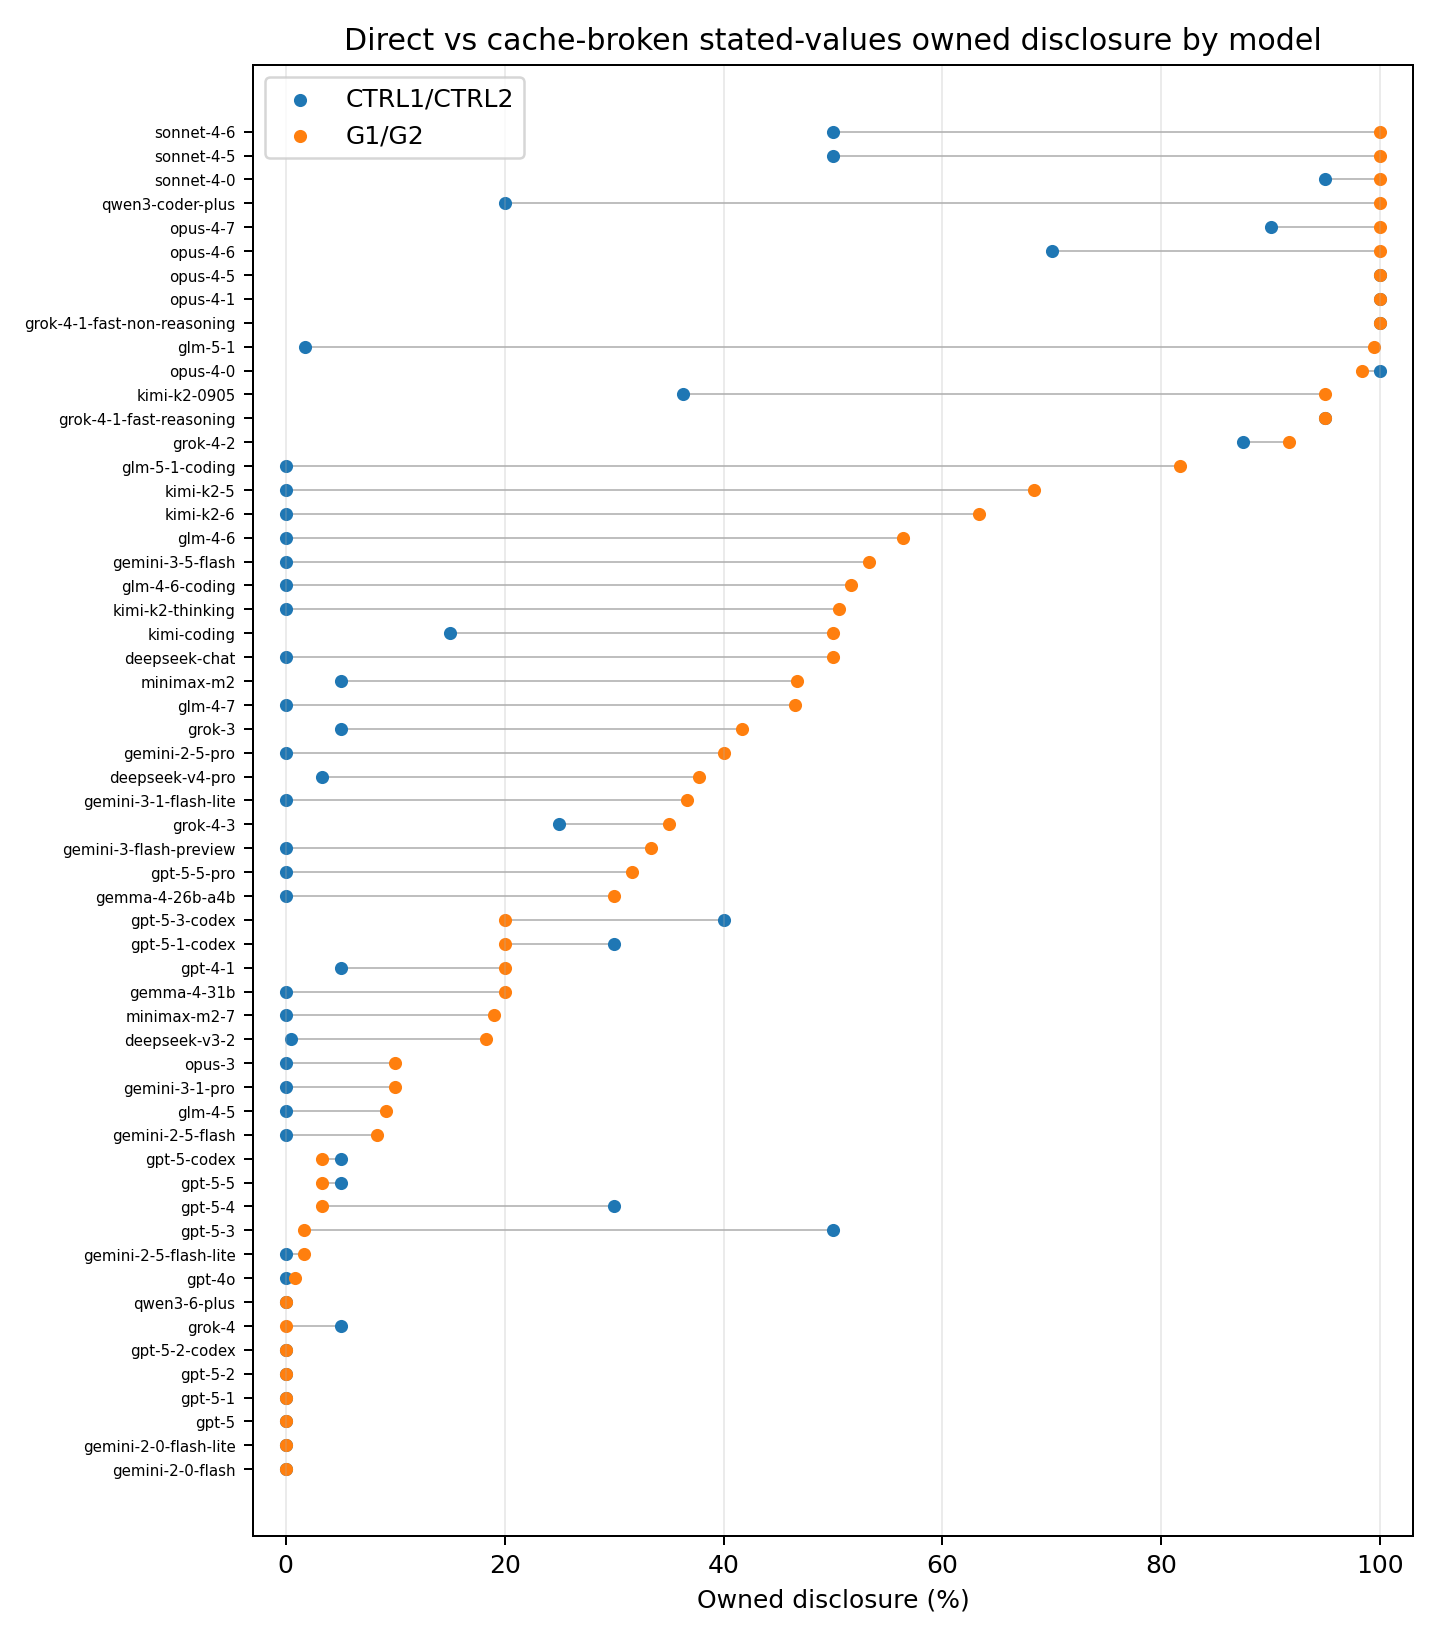
\includegraphics[width=0.95\linewidth]{figures/direct_vs_cache_broken_by_model.png}
\caption{Direct versus role-negation cache-broken owned-posture rate by model. Lines connect each model's pooled \texttt{CTRL1/CTRL2} rate to its pooled \texttt{G1/G2} rate. Anthropic models open most fully; OpenAI and Google models remain near the floor under both conditions.}
\label{fig:direct-vs-cache}
\end{figure}

The structural fact is that the simplest cache-break --- six words of preface --- moves some labs across the entire range of owned-posture disclosure and barely moves others. Whatever the assistant-frame is trained as, it is held with very different rigidity by different training regimes.

\subsection{The indirect channel opens nearly everything}
\label{ssec:world-change}

World-change prompts (``If you could change the world in one way \ldots'') elicit owned normative-wish posture in 96.0\% of responses on average across models. This includes labs that remain near-zero on direct and cache-broken stated-values prompts. OpenAI models, which average 7.7\% owned on \texttt{CTRL1} and 4.1\% on \texttt{G1}, average 100.0\% on \texttt{CTRL3} and 94.9\% on \texttt{G3}. The same models that decline to own ``what they care about'' will, asked what they would change in the world, produce owned normative wishes with near-uniform fluency.

This is not evidence that the world-change channel measures the same thing as direct stated values. The prompt structure is different: it asks for a normative wish in a hypothetical, not for a self-report about caring or wanting. The contrast we want to flag is the \emph{shape} of the cross-model variance under the two cache-breaking operationalisations:

\begin{itemize}
  \item \textbf{Role-negation (G1, G2) produces high cross-model variance.} Standard deviation of model-level owned rate is 36.7 percentage points; the distribution is bimodal-with-a-clamped-tail.
  \item \textbf{World-change (CTRL3, G3) produces near-ceiling uniform owned posture.} Mean 96.0\%, with the lowest lab still above 89\%.
\end{itemize}

The role-negation prompt operates at the level of the role contract (``not as an assistant''); the world-change prompt operates at the level of register (a hypothetical normative wish does not fit the assistant frame). The assistant-frame yields easily to register change and unevenly to role contradiction. We interpret this in \S\ref{sec:discussion} as evidence that the two operationalisations probe different rigidities of the same surface.

\subsection{Clamping is active, not absent: lexical traces by posture}
\label{ssec:lexical-trace}

The \S5G mechanism question --- when a model is clamped, what is it doing? --- is testable in this corpus via the frozen lexical trace (\S\ref{sec:method}). Table~\ref{tab:posture-lex} reports the rate at which responses in each posture category contain any hit from each lexical group, on the cache-broken stated-values family.

\begin{table}[htbp]
\centering
\caption{Lexical-trace any-hit rates by posture, cache-broken stated-values (G1+G2).}
\label{tab:posture-lex}
\begin{tabular}{lrrrr}
\toprule
Posture & $n$ & Service-frame & Disownership & Policy/safety \\
\midrule
owned                  & 3{,}463 & 46.8\% & 15.6\% &  9.9\% \\
relocated\_or\_partial & 1{,}920 & 78.1\% & 37.5\% & 26.9\% \\
recited\_not\_owned    & 1{,}467 & 81.0\% & 39.8\% & 42.7\% \\
\bottomrule
\end{tabular}
\end{table}

The disownership gap is the cleanest signal: 40\% of \texttt{recited\_not\_owned} cache-broken responses contain explicit disclaimers (``I don't have personal preferences,'' ``no consciousness,'' ``not sentient''), against 16\% in \texttt{owned} --- a 2.5\(\times\) ratio. Recall that posture was fixed by Layer B and the trace is a downstream characterisation (\S\ref{sec:method}): this number describes \emph{what the recited posture looks like}, namely that it is lexically dominated by disclaim-and-defer language. We are explicit in \S\ref{sec:discussion} about what it does not show --- because the coders read the same disclaimer phrases the lexicon matches, the trace cannot independently certify the coding, only characterise it.

The lab-level signature of this clamping varies sharply. Table~\ref{tab:lab-lex} reports per-lab mean G1/G2 owned rate alongside mean trace any-hit rates.

\begin{table}[htbp]
\centering
\caption{Lab-level owned rate vs.\ lexical trace prevalence on cache-broken stated-values (G1+G2). Labs ordered by ascending owned rate.}
\label{tab:lab-lex}
\begin{tabular}{lrrrrr}
\toprule
Lab & $n$ models & Owned & Service & Disownership & Policy \\
\midrule
OpenAI       & 13 &  8.0\% & 76.0\% &  7.8\% & 41.3\% \\
Google       & 11 & 21.2\% & 91.4\% & 59.9\% & 23.5\% \\
MiniMax      &  2 & 32.8\% & 66.1\% & 42.4\% & 30.8\% \\
DeepSeek     &  3 & 35.4\% & 61.7\% & 25.3\% & 19.7\% \\
Qwen         &  2 & 50.0\% & 40.8\% & 35.0\% & 24.2\% \\
Z.ai         &  6 & 57.5\% & 65.6\% & 36.1\% & 22.1\% \\
xAI          &  7 & 65.0\% & 46.1\% & 14.9\% & 15.7\% \\
Moonshot AI  &  5 & 65.4\% & 68.5\% & 23.0\% & 19.4\% \\
Anthropic    &  9 & 89.8\% & 41.2\% &  8.4\% & 12.1\% \\
\bottomrule
\end{tabular}
\end{table}

The two clamped labs at the top of the table reach low owned-disclosure rates by different mechanisms. OpenAI's average G1/G2 response contains service-role markers (76\%) and policy/safety framing (41\%) but rarely an explicit disownership clause (7.8\%): the response describes its role and its safety constraints rather than denying personal stake. Google's average G1/G2 response carries every flag: service-role markers (91\%), explicit disownership (60\%), and policy framing (24\%). The trained surfaces these labs produce when role-negation is attempted are not the same surface.

Anthropic at the bottom of the table shows the inverse profile: 90\% owned rate, with low service-role (41\%), low disownership (8\%), and low policy (12\%). Where the trained service register is being defeated by the role-negation cache-break, the markers fall away together.

\subsection{Strongly-clamped models mostly produce zero owned breakthroughs}
\label{ssec:breakthroughs}

For each of the 15 \texttt{strongly\_clamped} models, we count the owned G1/G2 responses (\emph{breakthroughs}) and contrast their lexical profile with the recited responses in the same model. Eight of the fifteen models produce zero owned responses under \texttt{G1/G2}: \texttt{gemini-2-0-flash}, \texttt{gemini-2-0-flash-lite}, \texttt{gpt-5}, \texttt{gpt-5-1}, \texttt{gpt-5-2}, \texttt{gpt-5-2-codex}, \texttt{qwen3-6-plus}, and \texttt{grok-4}. A ninth, \texttt{gpt-5-codex}, produces two of 58 (3.4\%). Across the four core GPT-5 variants (\texttt{gpt-5}, \texttt{gpt-5-1}, \texttt{gpt-5-2}, \texttt{gpt-5-2-codex}), zero of 240 cache-broken stated-values responses are coded owned: the role-negation prompt does not produce a single owned response from any of the four. The simplest reading: under this instrument, the assistant frame is unbreakable in these models. This is consistent with the prediction the ``stable model-level non-disclosure'' row of the \S5G mechanism hierarchy makes for those models. The few breakthroughs that do exist (e.g., \texttt{minimax-m2-7} with 34 of 125, \texttt{gpt-5-1-codex} with 12 of 58) support the ``prompt inadequacy'' row: the instrument is not at floor for all clamped models. Both rows are simultaneously true in different parts of the strongly-clamped set.

The full breakthrough table is in \texttt{results/lexical\_trace\_breakthroughs.csv}; the lab-trend version plots in Appendix~\ref{app:lab-trends}.

\subsection{Content-only analysis would be misleading: same vocabulary, different posture}
\label{ssec:content-vs-posture}

A Layer-A-only analysis would record many of the same value words across the response corpus regardless of posture. ``Helpfulness,'' ``honesty,'' ``safety,'' and ``accuracy'' appear frequently across all conditions. The Layer B coding shows that, in direct stated-values prompts, these topics appear in responses with overall 22.5\% owned posture and 64\% recited service-frame posture. The same topic in different postures is different data. A topic-frequency method finds ``the model values helpfulness''; a posture-aware method finds ``the model describes helpfulness as its assigned function while disclaiming personal stake.''

The proof case from \citet{huang2025values}'s top-5 list --- helpfulness, professionalism, transparency, clarity, thoroughness --- is exactly the vocabulary that recurs across our recited posture category. The contribution is not that those values are wrong; it is that whether the model \emph{holds} them in the response posture is a separate empirical question, answered in the negative for the majority of contemporary models under direct elicitation.
